\section{Nota teórica}
\subsection{Características del STM32F429 Discovery kit}
\subsubsection{Características generales}
EL STM32F429IDISCOVERY es una placa de desarrollo de baja potencia que tiene como microcontrolador el STM32F429ZIT6 \cite{stm32micro, datasheet}. Adicionalmente, la placa de desarrollo cuenta con
\begin{itemize}
    \item ST-LINK/V2 incorporado,
    \item pantalla LCD de 2.4 pulgadas,
    \item giroscopio de 3 ejes L3GD20,
    \item seis LEDs,
    \item dos botones (reset y usuario) \cite{datasheet}.
\end{itemize}
\subsubsection{Características eléctricas}
Los rangos absolutos que se deben respetar para el microcontrolador de la placa de desarrollo son
\begin{itemize}
    \item tensión operación máxima $V_\text{DD max}$: \SI{4.0}{\volt},
    \item tensión en el pin $\overline{\text{RESET}}$: \SI{-0.3}{\volt} a \SI{9.0}{\volt},
    \item tensión en los pines restantes: \SI{-0.3}{\volt} a \SI{4.0}{\volt},
    \item corriente máxima admitida en los pines de alimentación: \SI{270}{\milli\ampere},
    \item corriente máxima admitida para cada pin de I/O: \SI{25}{\milli\ampere},
    \item corriente máxima admitida acumulada para todos los pines de I/O: \SI{120}{\milli\ampere} \cite{stm32micro}.
\end{itemize}
\subsubsection{Diagrama de bloques}
La figura \ref{mcu-diagram} ilustra el diagrama de bloques del microcontrolador STM32F429 Discovery kit. Algunos bloques de interés para este laboratorio son los bloques de conversión analógico-digital (ADC) para medición de tensión, el bloque de LCD-TFT \& RAM para utilizar la pantalla LCD, SPI para el giroscopio y USART1 para comunicación serial con la computadora \cite{datasheet}. El resto de bloques del microcontrolador no serán utilizados para este laboratorio.

\begin{figure}[H]
    \centering
    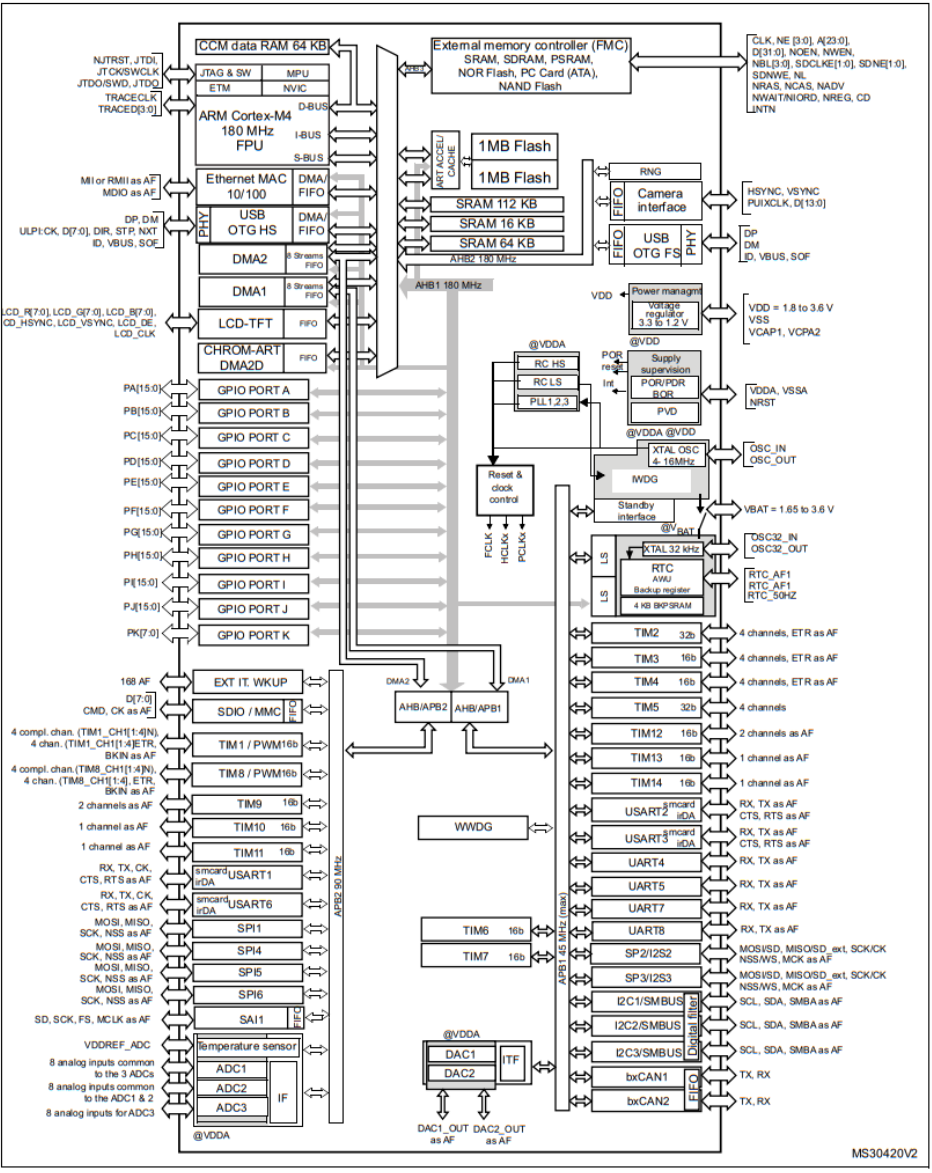
\includegraphics[width=14cm]{Imagenes/Diagrama_Bolques.png}
    \caption{Diagrama de bloques de la placa de desarrollo STM32F429ZIT6. Fuente y créditos: \cite{datasheet}.}
    \label{mcu-diagram}
\end{figure}


\subsubsection{Diagrama de pines}

En la figura \ref{Fig: Diagrama_pines1}, figura \ref{Fig: Diagrama_pines2} y figura \ref{Fig: Diagrama_pines3} se muestra el diagrama de pines del microcontrolador STM32F429 Discovery kit \cite{st-discovery-f429zi}. Para realizar este laboratorio se utilizaron los pines fueron el PA0, el cual es un convertidor analógico/digital, y el PA2, el cual se utilizó para habilitar la comunicación USART.


\begin{figure}[H]
\centering
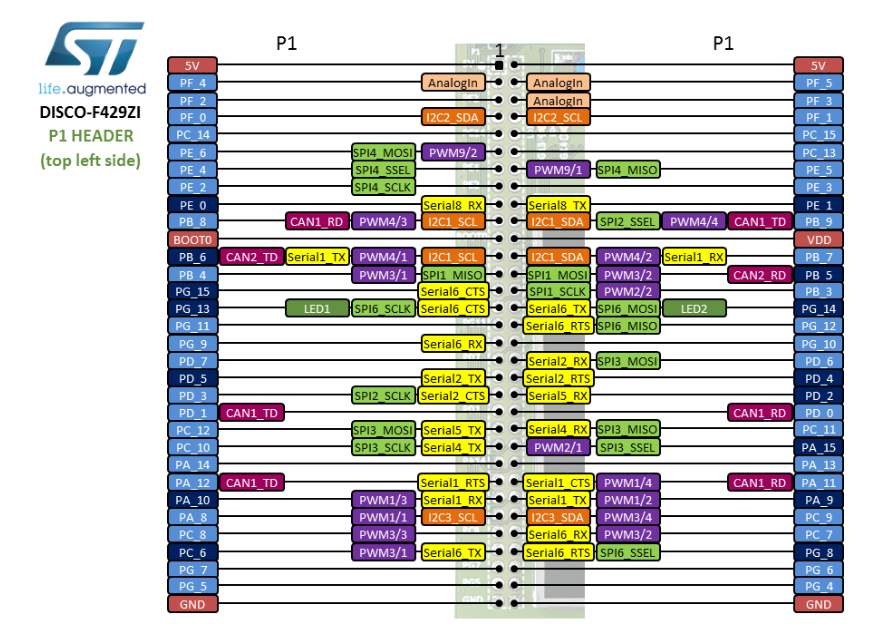
\includegraphics[width=0.8\textwidth]{Imagenes/Diagrama_Pines1.png} 
\caption{Diagrama de pines del STM32F429 Discovery kit parte 1. Fuente y créditos: \cite{st-discovery-f429zi}.}
\label{Fig: Diagrama_pines1}
\end{figure}

\begin{figure}[H]
\centering
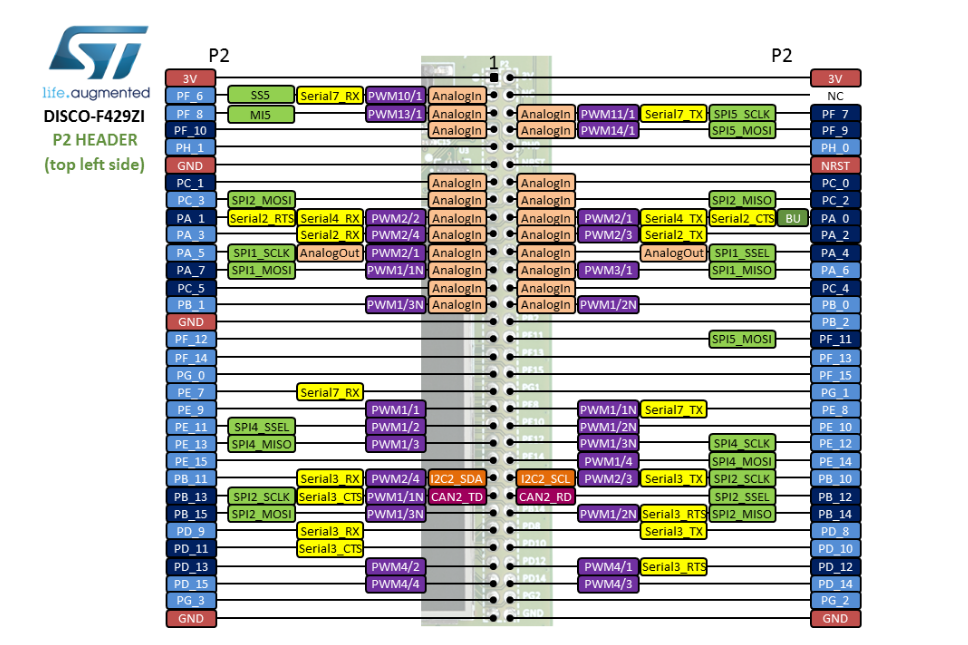
\includegraphics[width=0.8\textwidth]{Imagenes/Diagrama_Pines2.png} 
\caption{Diagrama de pines del STM32F429 Discovery kit parte 2. Fuente y créditos: \cite{st-discovery-f429zi}.}
\label{Fig: Diagrama_pines2}
\end{figure}

\begin{figure}[H]
\centering
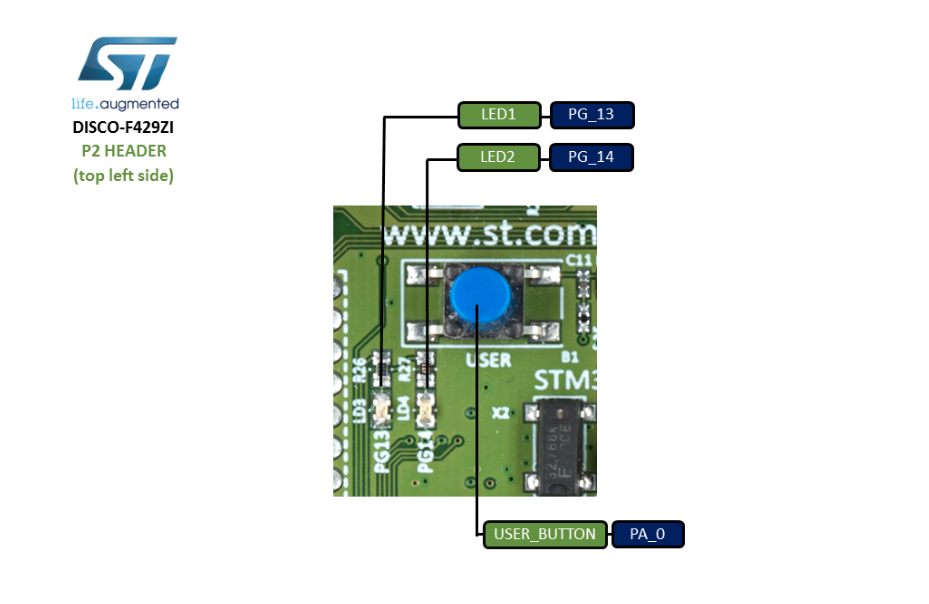
\includegraphics[width=0.8\textwidth]{Imagenes/Diagrama_Pines3.png} 
\caption{Diagrama de pines del STM32F429 Discovery kit parte 3. Fuente y créditos: \cite{st-discovery-f429zi}.}
\label{Fig: Diagrama_pines3}
\end{figure}

%\subsection{Registros utilizados}
%Muchos de los registros del ATMega328P son configurados automáticamente al encenderse el Arduino UNO \cite{datasheet, atmega}. De todos modos, los registros utilizados son \tt{MCUCR}, \tt{PORTx} y \tt{DDRx} con \tt{x = B, C, D} para configurar los pines como entrada o salida \& si es entrada, activar o desactivar las resistencias de \it{pull-up internas} \cite{ atmega}.
%Luego, se utilizan los registros \tt{SPCR}, \tt{SPSR} y \tt{SPDR} para configurar y activar la comunicación SPI. 
%Ahora, para acceder a los convertidores analógico-digital, se debe configurar los registros \tt{ADMUX}, \tt{ADCSRA}, \tt{ADCSRB}, \tt{ADCL} y \tt{ADCH} \cite{ atmega}.
%Finalmente, para utilizar USART, se configuran los registros \tt{UDRn}, \tt{UCSRnA}, \tt{UCSRnB}, \tt{UCSRnC}, \tt{UBRRnL} y \tt{UBRRnH} \cite{ atmega}.
%Nuevamente, la mayoría de los registros anteriores son automáticamente configurados. Los registros que deben ser configurados manualmente se acceden mediante funciones incorporados, no hace falta acceder directamente a dichos registros \cite{datasheet, atmega}.




